\chapter{Aspekt bezpieczeństwa w systemach rekomendacyjnych}
Systemy rekomendacyjne muszą gromadzić wiele danych o użytkownikach w celu wykonania trafnego przewidywania potencjalnych obiektów zainteresowania. W zależności od metody serwis dokonuje porównania  profili użytkowników, oblicza podobieństwo pomiędzy użytkownikami czy grupuje użytkowników o zbliżonych cechach. Gromadzone w tym celu dane mogą pozwolić na identyfikacje użytkownika przez co twórcy systemu muszą wybierać pomiędzy prywatnością użytkowników, a skutecznością w dokonywaniu rekomendacji. Taki system z wrażliwymi danymi użytkowników może stać się celem grup hakerskich chcących pozyskać tak cenne informacje. Stąd zapewnienie bezpieczeństwa podczas przesyłania danych pomiędzy serwisami oraz dokonywania obliczeń na nich powinno stać się priorytetem. Jednak większość prac skupia się na zwiększeniu skuteczności czy wydajności \cite{recent_developments}.

\section{Prywatność}
Prywatność w kontekście systemów rekomendacyjnych oznacza, że podczas pracy systemy żadne dane nie mogą wyciec, a także otrzymana predykcja nie powinna pozwolić na identyfikację użytkownika. Na rysunku \ref{fig:podatnosci} przedstawiono potencjalne miejsca, w których dane mogą zostać przechwycone. Jak widać atakujący mogą uzyskać dane podczas wprowadzania ich do systemu, przesyłania ich pomiędzy poszczególnymi komponentami usługi, jak i w trakcie wysłania predykcji do użytkownika. Idealny, zachowujący prywatność system rekomendacyjny powinien być bezpieczny bez znaczącej utraty na wydajności jako całości, a przede wszystkim bez zmniejszenia trafności rekomendacji. Systemy rekomendacyjne muszą stawić czoła ochronie prywatności użytkowników jak i ochronie wszystkich uczestników procesu rekomendacji. Wiele technik uczenia maszynowego w celu zachowania prywatności skupia się na wykorzystaniu wielu części do wspólnego trenowania modelu bez dzielenia się swoimi danymi w oryginalnej formie (dane są przesyłane wyłącznie w sposób zaszyfrowany). Osiąga się to poprzez:
\begin{itemize}
    \item perturbacje danych (ang. \textit{data perturbation}),
    \item bezpieczne obliczenia wieloczęściowe (ang. \textit{secure multiparty computation}).
\end{itemize}

\begin{figure}
    \centering
    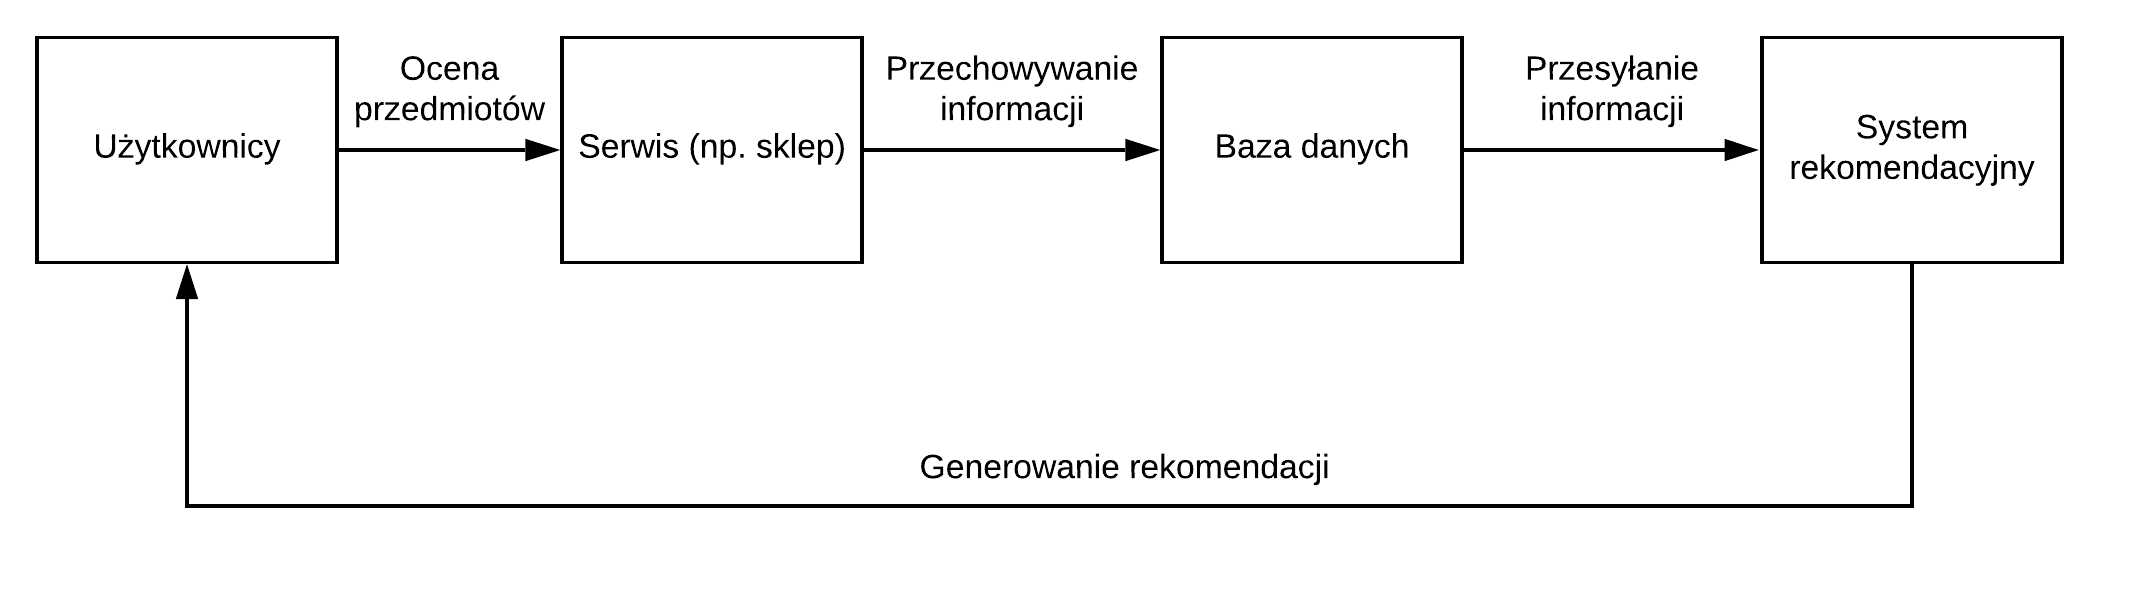
\includegraphics[scale=0.85]{images/podatnosci.png}
    \caption{Potencjalne podatności systemu.}    Źródło: opracowanie własne na podstawie \cite{practicalPrivacy}

    \label{fig:podatnosci}
\end{figure}
\section{Perturbacja danych}
Właściciel danych (użytkownik) dokonuje perturbacji własnych danych poprzez dodanie losowego szumu, a następnie przesyła je w celu dalszego przetwarzania.
Możemy wyróżnić następujące rodzaje perturbacji danych:
\begin{itemize}
    \item addytywne - opisane następującym wzorem 
    Y = X + C, gdzie C jest szumem dodanym do oryginalnej macierzy X. W praktyce każdy wiersz C generowany jest niezależnie,
    \item multiplikatywne - opisane wzorem Y = MX, gdzie M jest to macierz przez którą przekształcana są dane źródłowe. W przypadku tej metody nie ma gwarancji, że zostanie zachowana prywatność (przypadek w którym atakujący zna porcję danych w zbiorze X oraz ich odpowiednik w zbiorze M),
    \item prywatność różnicowa - wyróżnia się trzy podejścia w zależności od momentu wprowadzenia szumu: do danych wejściowych, w trakcie przetwarzania lub do danych wyjściowych.
\end{itemize}

Natomiast ze względu na miejsce gdzie dochodzi i jak do perturbacji danych podział wygląda następująco \cite{PPML}:
\begin{itemize}
    \item perturbacja wejścia - szum dodawany jest do danych,
    \item perturbacja algorytmu - dodanie szumu dochodzi pomiędzy iteracjami danego algorytmu,
    \item perturbacja wyjścia - na danych wejściowych uruchamiany jest algorytm niezachowujący prywatności, a następnie do uzyskanego rezultatu dodawany jest szum,
    \item obiektywna perturbacja - szum dodawany jest do funkcji obiektywnej (funkcja używana do optymalizacji problemu).
\end{itemize}

Głównym problemem w wykorzystaniu perturbacji danych w celu zapewnienia prywatności jest brak gwarancji, że uzyskane wyniki będą tak samo trafne jak w przypadku bez wprowadzenia szumu w danych. Dodanie zbyt dużego szumu może powodować niską jakość wskazywania podobnych użytkowników lub przedmiotów.



\section{Bezpieczne obliczanie wieloczęściowe}

Metoda pozwala rozproszonym stronom na wspólne obliczanie bez konieczności odkrywania ich prywatnych danych wejściowych oraz wyjściowych. Ponadto zastosowania obliczania wieloczęściowego nie wymaga użycia zaufanej trzeciej strony (bezpieczeństwo pozostaje takie samo jak w przypadku wykorzystania trzeciej strony). 
Wyróżniane są następujące rozwiązania:
\begin{itemize}
    \item rozwiązania oparte na bezpiecznym dodawaniu wektorów (\textit{ang. Secure Vector Addition based Solutions}),
    \item szyfrowanie homomorficzne - pozwala na wykonywanie operacji (dodawanie, mnożenie) na zaszyfrowanych danych, bez konieczności ich deszyfrowania. Ze względu na wysoki koszt związany z wykonywanymi operacjami, w modelach uczenia maszynowego wykorzystuje się częściej dodawanie,
    \item podejścia oparte na bezpiecznych produktach skalarnych (\textit{ang. Secure scalar product based approach}) - umożliwia na obliczanie przez strony iloczynu skalarnego ich prywatnych wektorów, bez ich przekazywania. Metoda wykorzystywana przede wszystkim w celu eksploracji danych oraz analizie statystycznej,
    \item podejścia oparte o "zniekształcony obwód" (\textit{ang. Garbled circuit based approach}) - jedna ze stron przesyła funkcję obliczeniową w postaci obwodu, w ten sposób druga strona może użyć tej samej funkcji w celu wykonania obliczeń na własnych danych.
\end{itemize}

W celu wykorzystania bezpiecznego obliczania wieloczęściowego powstały specjalne bibliotek takie jak: CrypTFlow (nakładka na bibliotekę Tensorflow składająca się z trzech komponentów - Athos, Porthos i Aramis) \cite{kumar2020cryptflow} czy EzPC \cite{chandran2019ezpc}.

Z powodu wysokiego kosztu obliczeniowego bezpieczne obliczanie wieloczęściowe nie zawsze znajdują zastosowanie w komercyjnych rozwiązaniach związanych z rekomendacją. Spowodowane jest tym, że metody te na ten moment nie mogą być rozpatrywane przy systemach wymagających działania w czasie rzeczywistym. \cite{secureMultipartyComputation}

\section{Federated learning}
\label{section:federatedLearning}

Pojęcie wprowadzone przez firmę Google w 2016 roku. Standardowe uczenie maszynowe zakłada, że dane treningowe znajdują się na jednej maszynie lub w centrum danych. Model \textit{Federated learning} umożliwia na wspólne uczenie z udostępnianego wcześniej wyuczonego modelu bez dzielenia się prywatnymi danymi z innymi użytkownikami bądź z scentralizowanym serwerem, a także nie wymaga przechowywania danych po stronie serwera.

Uproszczony opis działania algorytmu (na rys. \ref{fig:fl} przedstawiono schemat):
\begin{enumerate}
    \item Urządzenie (na przykład smartphone) pobiera wcześniej wytrenowany model.
    \item Model jest aktualizowany (ponownie trenowany na danych znajdujących się na urządzeniu) (A).
    \item Aktualizacja modelu wysyłana jest do chmury poprzez zaszyfrowaną komunikację.
    \item Aktualizacja jest uśredniana z pozostałymi aktualizacjami modelu otrzymanymi od innych użytkowników (B).
    \item Model jest aktualizowany na bazie uśrednionych wyników (C).
\end{enumerate}

\begin{figure}
    \centering
    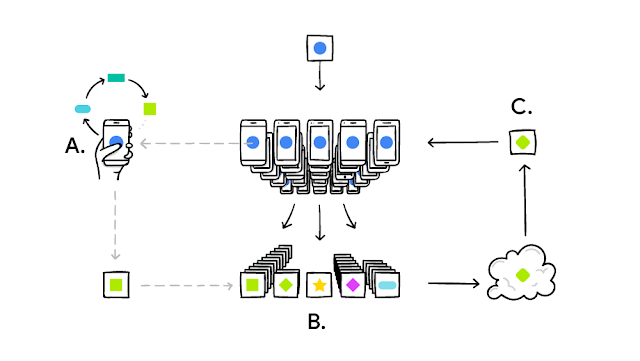
\includegraphics[scale=0.6]{images/fl.png}
    \caption{Schemat działania \textit{Federated Learning}.}    Źródło: Google AI Blog \cite{fedderatedLearning}
    \label{fig:fl}
\end{figure}

\textit{Federated learning} wykorzystywane jest tam gdzie dane są wrażliwe lub ilość danych jest na tyle duża, że przesłanie ich do jednego zbiorczego kontenera jest nieopłacalne. Przykładowymi zastosowaniami są między innymi w \textit{Google GBoard} \cite{fedderatedLearning} - wirtualna klawiatura przewidująca kolejne słowa użytkownika, w badaniach farmaceutycznych \cite{fedderatedLearningHealth} czy w samochodach autonomicznych \cite{fedderatedLearningVehicle}.

Zastosowanie tego rozwiązania umożliwia na zmniejszenie czasu przetwarzania danych poprzez nie wysyłanie ich w stanie surowym do serwera, a procesowanie danych bezpośrednio na urządzeniu, które zebrało dane. Zastosowanie tej technologii nie wymaga stałego połączenia z Internetem, a także nie wymaga dodatkowej infrastruktury sprzętowej do sprawnej komunikacji czy wykonywania obliczeń

Mimo szeregu zalet zastosowanie tego modelu wymaga częstej komunikacji pomiędzy poszczególnymi węzłami uczącymi. Oprócz dobrej wydajności sprzętu i pamięci, ważne jest także zapewnienie wysokiej przepustowości łącza w celu wymiany uzyskanych wyników. Kolejną wadą jest fakt, że nie ma pewności co do jakości danych na których generowany jest model. Jeżeli te dane skrajnie odbiegają od pozostałych może to spowodować znaczącą zmianę głównego modelu.

\section{Przegląd aktualnych rozwiązań}

W \cite{practicalPrivacy} zaprezentowano schemat składający się z dwóch faz. W pierwszej fazie użytkownicy szyfrują swoje oceny oraz przesyłają szyfrogram do serwera. Serwer korzystając z właściwości homomorficznych (obliczenia na zaszyfrowanych danych) oblicza podobieństwa i średnie, które następnie są przechowywane w bazie. Druga faza to generowanie rekomendacji w której użytkownik na podstawie wysłanych zaszyfrowanych danych otrzymuje od serwera rekomendacje, które może odszyfrować wyłącznie on za pomocą prywatnego klucza. Proponowane rozwiązanie dotyczy zarówno metody \textit{Content-based Filtering} jak i \textit{Collaborative filtering}.

Inne mechanizmy zaproponowano w \cite{contributionsToSecurityRS}. W pierwszym podejściu ograniczono ilość wymaganych danych przesyłanych przez użytkownika, co powoduje niestety zmniejszenie liczby wymiarów, które są wykorzystywane do rekomendacji. Drugim podejściem jest protokół komunikacyjny umożliwiający na obliczenie podobieństwa użytkowników bazując na dowodach o wiedzy zerowej (jedna ze stron może udowodnić, że posiada daną informację bez jej ujawniania). Podczas wymiany dwóch użytkowników starają się wyłącznie dowiedzieć czy są do siebie podobnie. Według autora zaprezentowane podejścia mogą być ze sobą połączone jednocześnie.

Natomiast w \cite{weakTies} przedstawiono zastosowanie \textit{weak ties}, które są nieoczywistymi połączeniami między użytkownikami dające trafne rekomendacje. W tym celu zastosowano model \textit{jumping connections}, który dokonuje rekomendacji poprzez serię skoków pomiędzy użytkownikami (w najbliższym sąsiedztwie rekomendacji występuje jedynie jeden skok).

